\section{Algoritmos de Ejecución: Memoria Condicional, Embeddings, Estabilidad y Enrutamiento de Inferencia}
\label{sec:annex-runtime}

Este anexo recopila los algoritmos de ejecución que soportan la tubería impulsada por configuración: memoria condicional (Engram), embeddings factorizados y convolución de embedding, controles de estabilidad del paso de entrenamiento, la partición de evaluación reservada y el enrutador de modo de inferencia SBERT. Las claves bibliográficas citadas aquí se resuelven contra \texttt{docs/bibliography/}.

\subsection{Memoria Condicional Engram}

\begin{figure}[H]
\centering
\fitfigure{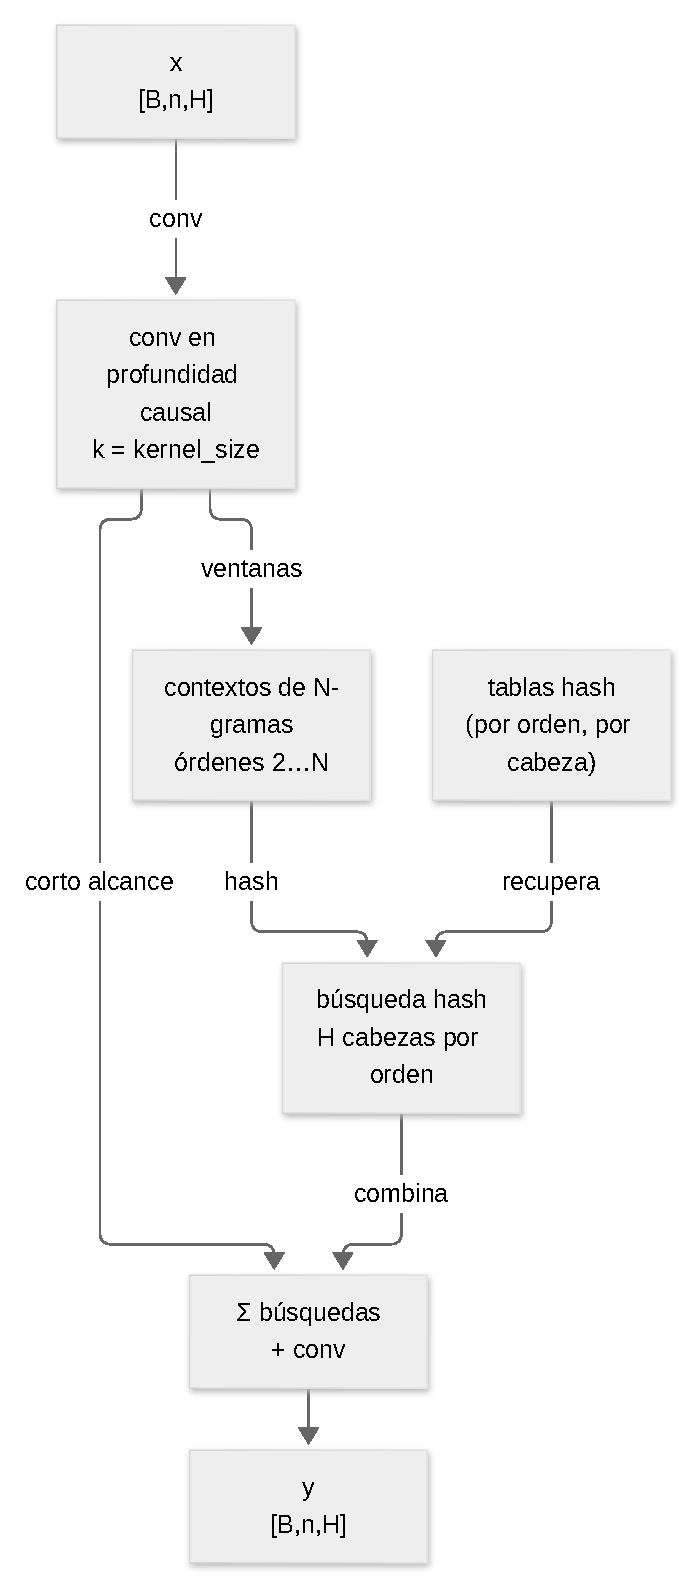
\includegraphics{../paper/figures/mixers/engram-es.pdf}}
\caption{Flujo de datos de la memoria condicional de Engram: una convolución causal depthwise aporta contexto de corto alcance, las búsquedas hash de N-gramas recuperan embeddings por orden, y las búsquedas se suman a la salida de la convolución.}
\label{fig:mixer-engram}
\end{figure}

Engram (\texttt{engram}) implementa memoria condicional mediante búsqueda N-gram escalable \citep{cheng2026conditionalmemoryscalablelookup}. Construye tablas de búsqueda basadas en hash para contextos N-gram desde tamaño 2 hasta \texttt{engram\_max\_ngram\_size}, con cabezas hash independientes por orden N-gram. Una convolución causal depthwise (\texttt{engram\_kernel\_size}) proporciona contexto de corto alcance antes de la búsqueda N-gram.

\begin{algorithmic}[1]
\State \textbf{Entrada:} flujo de tokens $x_{1:n}$, órdenes N-gram $\{2, \ldots, N\}$, cabezas hash por orden $H$
\State $h_{\text{conv}} \gets \text{DepthwiseConv1d}(x_{1:n}, k=\texttt{engram\_kernel\_size})$ \Comment{contexto de corto alcance}
\For{cada orden N-gram $k \in \{2, \ldots, N\}$}
    \State $\text{ctx}_t^{(k)} \gets x_{t-k+1:t}$ \Comment{ventana de contexto N-gram}
    \State $\text{lookup}^{(k)}_t \gets \text{HashTable}^{(k)}[\text{hash}(\text{ctx}_t^{(k)})]$ \Comment{recuperación por cabeza, $H$ cabezas por orden}
\EndFor
\State $y_t \gets \sum_{k} \text{lookup}^{(k)}_t + h_{\text{conv},t}$ \Comment{combinar memorias condicionales}
\State \textbf{Salida:} $y_{1:n}$
\end{algorithmic}

\subsubsection{Configuración}
\begin{itemize}[leftmargin=*]
    \item \texttt{engram\_max\_ngram\_size}: int $\ge 2$ --- orden N-gram más alto (por defecto 3).
    \item \texttt{engram\_n\_heads\_per\_ngram}: int $\ge 1$ --- cabezas hash por orden N-gram (por defecto 4).
    \item \texttt{engram\_embed\_dim\_per\_head}: int $\ge 1$ --- dimensión de embedding por cabeza hash (por defecto 32).
    \item \texttt{engram\_kernel\_size}: int $\ge 1$ --- ancho del kernel de conv causal depthwise (por defecto 4).
    \item \texttt{engram\_seed}: int --- semilla hash para reproducibilidad (por defecto 42).
\end{itemize}
Tamaño oculto total de Engram = $(\texttt{max\_ngram\_size} - 1) \times \texttt{n\_heads\_per\_ngram} \times \texttt{embed\_dim\_per\_head}$.

\subsection{Embeddings Factorizados y Convolución de Embedding}

\subsubsection{Embeddings Factorizados}
Cuando \texttt{use\_factorized\_embedding=true}, la matriz de embedding se factoriza en dos matrices más pequeñas, reduciendo parámetros de $O(V \times H)$ a $O(V \times R + R \times H)$ donde $R = \texttt{factorized\_embedding\_dim}$.
\begin{itemize}[leftmargin=*]
    \item \texttt{use\_factorized\_embedding}: bool --- habilitar factorización.
    \item \texttt{factorized\_embedding\_dim}: int $\ge 1$ --- dimensión intermedia (típico: 64--256).
\end{itemize}

\subsubsection{Convolución de Embedding}
Cuando \texttt{use\_embedding\_conv=true}, se aplica una Conv1d depthwise sobre el flujo de embeddings antes del primer bloque transformer, con tamaño de kernel \texttt{embedding\_conv\_kernel}. Esto proporciona un filtro ligero de contexto local sobre embeddings de tokens.

\subsection{Controles de Estabilidad del Paso de Entrenamiento}

El paso de entrenamiento guiado por esquema aplica acumulación de gradientes, recorte de norma global, guardas de explosión post-recorte y reintentos acotados de NaN/Inf. El gradiente acumulado es:
\[
g_{\text{acc}}=\frac{1}{K}\sum_{i=1}^{K} g_i,\quad K=\texttt{gradient\_accumulation\_steps}
\]
\[
g_{\text{clip}} = g_{\text{acc}}\cdot
\min\left(1,\frac{\tau}{\|g_{\text{acc}}\|_2+\epsilon}\right),\quad
\tau=\texttt{grad\_clip\_max\_norm}
\]
luego los guardas de desbordamiento usan \texttt{inf\_post\_clip\_threshold} y lógica de reintentos limitada por \texttt{max\_nan\_retries}.

\begin{algorithm}[t]
\caption{Paso de Entrenamiento Guiado por Esquema con Controles de Estabilidad}
\begin{algorithmic}[1]
\Require Flujo de lotes, configuración $C$
\State Inicializar contador de reintentos $r\gets 0$
\For{cada paso del optimizador}
    \State Acumular gradientes para $K=C.\texttt{gradient\_accumulation\_steps}$ micro-lotes
    \State Aplicar recorte de norma global con $\tau=C.\texttt{grad\_clip\_max\_norm}$
    \If{el gradiente post-recorte excede $C.\texttt{inf\_post\_clip\_threshold}$ o se detecta NaN/Inf}
        \If{$r < C.\texttt{max\_nan\_retries}$}
            \State restaurar estado seguro / saltar paso; $r \gets r+1$
            \State \textbf{continue}
        \Else
            \State detener entrenamiento con estado de fallo
        \EndIf
    \EndIf
    \State ejecutar paso del optimizador seleccionado por \texttt{optimizer\_class}
    \State actualizar scheduler (\texttt{cosine}, \texttt{constant}, o \texttt{linear\_warmup\_then\_constant})
    \If{paso mod \texttt{checkpoint\_every\_n\_steps}$=0$}
        \State guardar checkpoint rodante y podar a \texttt{max\_rolling\_checkpoints}
    \EndIf
    \State actualizar mejores checkpoints hasta \texttt{num\_best\_checkpoints}
    \State emitir CSV + telemetría según \texttt{gradient\_log\_interval} y \texttt{telemetry\_log\_interval}
\EndFor
\end{algorithmic}
\end{algorithm}

\subsection{Partición de Test Reservada y Evaluación al Final del Entrenamiento}

\texttt{training.test\_percentage} reserva una fracción determinista del dataset de la tarea antes del primer paso del optimizador. Con $n$ ejemplos, porcentaje reservado $\rho=\texttt{test\_percentage}/100$ y una permutación $\pi$ sorteada una sola vez con la semilla de la ejecución \texttt{training.seed}, la partición es
\[
n_{\text{test}}=\operatorname{clip}\!\left(\operatorname{round}(\rho n),\,1,\,n-1\right),\qquad
\mathcal{D}_{\text{train}}=\{x_{\pi(i)}\}_{i=n_{\text{test}}+1}^{n},\qquad
\mathcal{D}_{\text{test}}=\{x_{\pi(i)}\}_{i=1}^{n_{\text{test}}} ,
\]
de modo que la misma configuración siempre reserva los mismos ejemplos, sea cual sea el mezclado del DataLoader. Tras la última época se evalúan los pesos finales una vez con el objetivo de la tarea bajo \texttt{no\_grad}, y la pérdida y precisión ponderadas por muestra
\[
\hat{L}=\frac{1}{n_{\text{test}}}\sum_{x\in\mathcal{D}_{\text{test}}}\ell(f_\theta;x),\qquad
\widehat{\text{acc}}=\frac{1}{n_{\text{test}}}\sum_{x\in\mathcal{D}_{\text{test}}}a(f_\theta;x)
\]
se escriben en \texttt{test\_metrics.json} junto al log CSV. La partición cubre modelado de lenguaje enmascarado y causal, clasificación de texto, las tres tareas de visión, ASR (donde el campo de precisión lleva la tasa de error de caracteres, etiquetada \texttt{metric: cer}) y clasificación de audio. SBERT conserva su propia partición de validación mediante \texttt{training.sbert.max\_eval\_samples} y no se ve afectado. Fijar el campo en cero desactiva la partición y restaura el comportamiento histórico sobre todos los datos.

\subsection{Enrutador de Modo de Inferencia SBERT}

El despachador de inferencia SBERT selecciona entre puntuación de similitud, búsqueda sobre corpus, agrupamiento y codificación persistente sobre un único codificador compartido \citep{reimers_sentence-bert_2019}. La similitud coseno y la pérdida de regresión son:
\[
\text{cos}(e_1,e_2)=\frac{e_1^\top e_2}{\|e_1\|\|e_2\|},\qquad
\mathcal{L}_{\text{cos}}=\left(\text{cos}(e_1,e_2)-y\right)^2
\]
con $y\in[-1,1]$ en este pipeline.

\begin{algorithm}[t]
\caption{Enrutador de Modo de Inferencia SBERT}
\begin{algorithmic}[1]
\Require modo $m$, modelo $E$, entradas $X$
\If{$m=\texttt{similarity}$}
    \State retornar $\cos(E(x_1),E(x_2))$
\ElsIf{$m=\texttt{search}$}
    \State retornar top-$k$ por producto-punto/coseno contra embeddings del corpus
\ElsIf{$m=\texttt{cluster}$}
    \State retornar etiquetas de clustering sobre $E(X)$
\Else
    \State retornar embeddings serializados $E(X)$
\EndIf
\end{algorithmic}
\end{algorithm}